\section{Casi d'uso}
    \subsection{Attori dei casi d'uso}
    \subsubsection{Attori primari}
    Gli attori che il gruppo ha ritenuto essere i più adeguati sono:
        \begin{itemize}
            \item \textbf{Utente generico:} si divide in:
                \begin{itemize}
                    \item \textbf{Utente non autenticato:} utente che può navigare nell'e-commerce e può usufruire di alcune funzionalità, come la visualizzazione e la ricerca dei prodotti, che può aggiungere al proprio carrello, la applicazione di filtri e categorie per la ricerca, e infine di potersi autenticare.
                    \item \textbf{Utente autenticato:} un utente autenticato può a sua volta essere:
                        \begin{itemize}
                            \item \textbf{Cliente autenticato:} cliente che ha effettuato il login, può accedere a molte funzionalità, come l'aggiunta di prodotti al carrello, l'acquisto, la visualizzazione della lista degli ordini, la possibilità di contattare il venditore;
                            \item \textbf{Venditore autenticato:} venditore che ha effettuato il login, può accedere alle funzionalità relative all'amministrazione dei prodotti e delle categorie.
                        \end{itemize}
                        \begin{figure}[!ht]
                            \caption{Attori primari}
                            \vspace{5px}
                            
\includegraphics[scale=0.59]{../../../Images/attori}
                            \centering
                        \end{figure}
                \end{itemize}
        \end{itemize}
    \subsection{Elenco dei casi d'uso}
        \textbf{Utilizzo della piattaforma:}
        \begin{figure}[!ht]
            \caption{Casi d'uso che interessano gli utenti}
            \vspace{10px}
            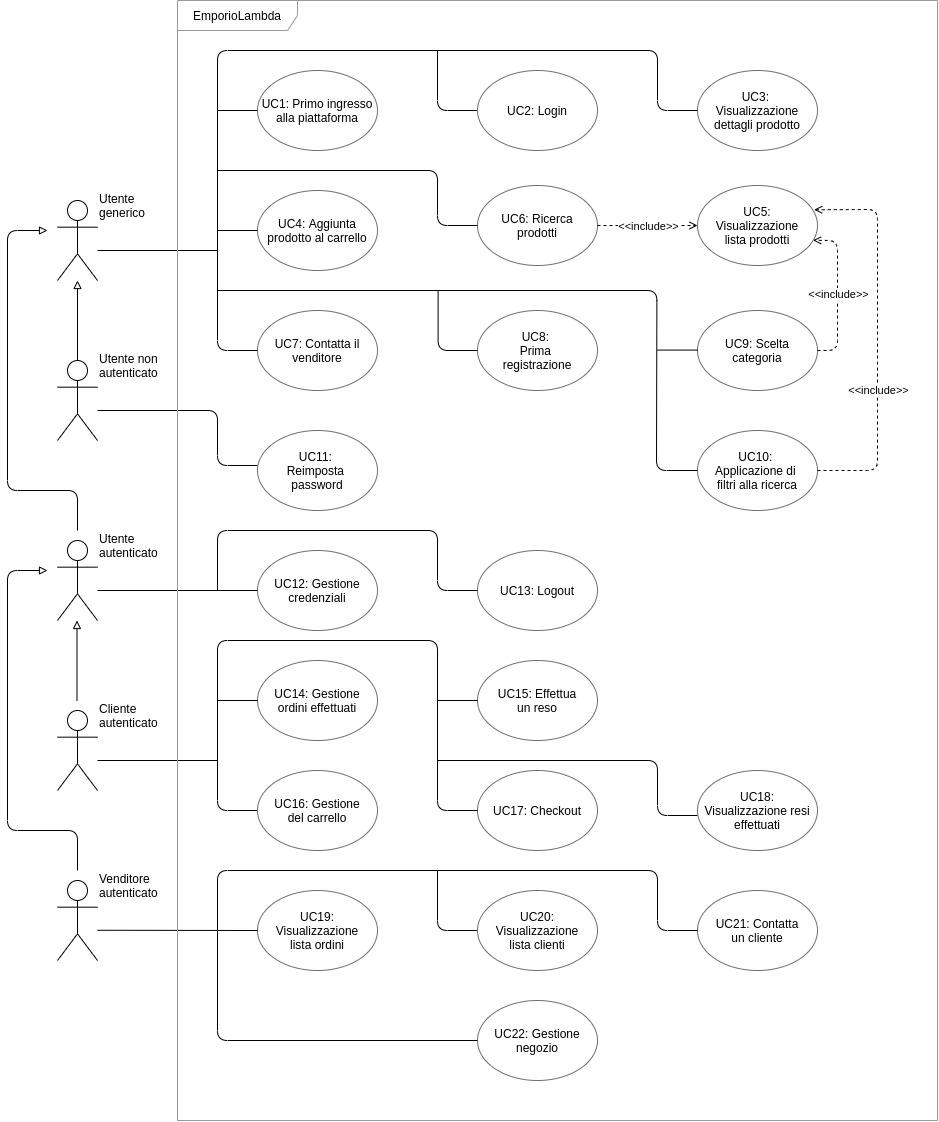
\includegraphics[scale=0.5]{../../../Images/casiUso.png}
            \centering
        \end{figure}
        \subsection{UC1: Primo ingresso alla piattaforma}
        \subsection{UC2: Login}
        \subsection{UC3: visualizzazione dettagli di un prodotto}
        \subsection{UC4: Aggiunta di un prodotto al carrello}
        \subsection{UC5: Ricerca dei prodotti}
        \subsection{UC6: Visualizzazione della lista dei prodotti}
        \subsection{UC7: Contatta il venditore}
        \subsection{UC8: Prima registrazion<e}
        \subsection{UC9: Scelta della categoria}
        \subsection{UC10: Applicazione dei filtri alla ricerca}
        \subsection{UC11: Reimposta password (dimenticata)}
        \subsection{UC12: Gestione credenziali}
        \subsection{UC13: Logout}
        \subsection{UC14: Gestione degli ordini effettuati}
        \subsection{UC15: Effettua un reso}
        \subsection{UC16: Gestione del carrello}
        \subsection{UC17: Checkout}
        \subsection{UC18: Visualizzazione dei resi effettuati}
        \subsection{UC19: Visualizzazione della lista degli ordini}
        \subsection{UC20: Visualizzazione della lista degli utenti}
        \subsection{UC21: Contatta un cliente}
        \subsection{UC22: Gestione del negozio}

